\documentclass{standalone}
\usepackage{tikz}
\usetikzlibrary{patterns, positioning}
\usepackage[sfdefault]{ClearSans} %% option 'sfdefault' activates Clear Sans as the default text font
\usepackage[T1]{fontenc}

\begin{document}
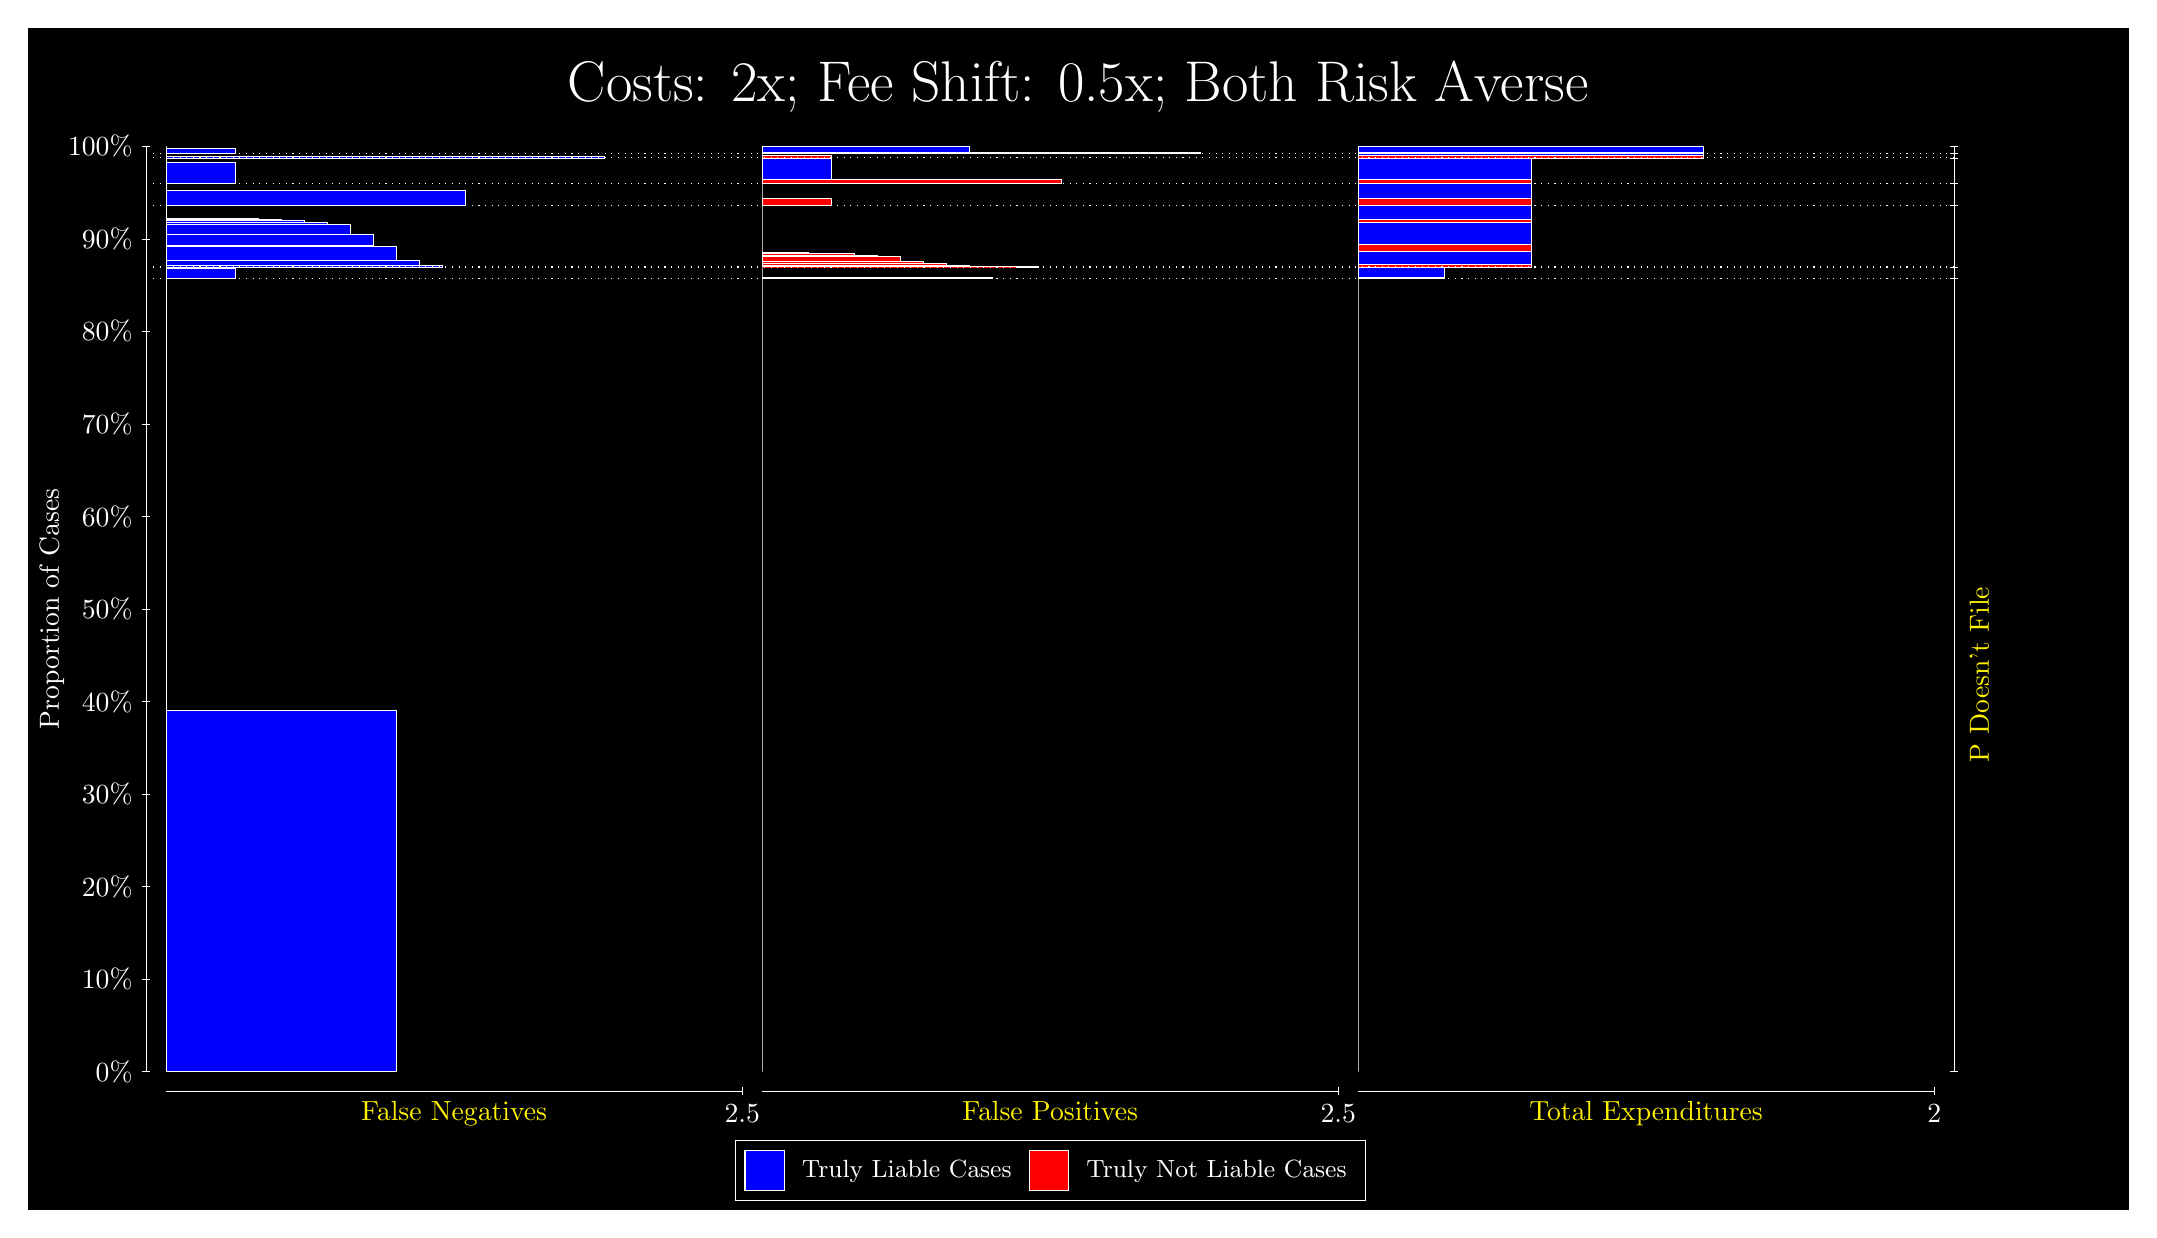
\begin{tikzpicture}
\draw[fill=black] (0,0) rectangle (26.667,15);
\draw[text=white] (0,13.5) rectangle (26.667,15) node[midway] {\huge Costs: 2x; Fee Shift: 0.5x; Both Risk Averse};
\draw[white, very thin] (1.5,1.75) -- (1.5,13.5);
\node[rotate=90, text=white, anchor=center] at (0.3, 7.625) {Proportion of Cases};
\draw[white, very thin] (1.45,1.75) -- (1.55,1.75);
\node[text=white, anchor=east] at (1.45, 1.75) {0\%};
\draw[white, very thin] (1.45,2.925) -- (1.55,2.925);
\node[text=white, anchor=east] at (1.45, 2.925) {10\%};
\draw[white, very thin] (1.45,4.1) -- (1.55,4.1);
\node[text=white, anchor=east] at (1.45, 4.1) {20\%};
\draw[white, very thin] (1.45,5.275) -- (1.55,5.275);
\node[text=white, anchor=east] at (1.45, 5.275) {30\%};
\draw[white, very thin] (1.45,6.45) -- (1.55,6.45);
\node[text=white, anchor=east] at (1.45, 6.45) {40\%};
\draw[white, very thin] (1.45,7.625) -- (1.55,7.625);
\node[text=white, anchor=east] at (1.45, 7.625) {50\%};
\draw[white, very thin] (1.45,8.8) -- (1.55,8.8);
\node[text=white, anchor=east] at (1.45, 8.8) {60\%};
\draw[white, very thin] (1.45,9.975) -- (1.55,9.975);
\node[text=white, anchor=east] at (1.45, 9.975) {70\%};
\draw[white, very thin] (1.45,11.15) -- (1.55,11.15);
\node[text=white, anchor=east] at (1.45, 11.15) {80\%};
\draw[white, very thin] (1.45,12.325) -- (1.55,12.325);
\node[text=white, anchor=east] at (1.45, 12.325) {90\%};
\draw[white, very thin] (1.45,13.5) -- (1.55,13.5);
\node[text=white, anchor=east] at (1.45, 13.5) {100\%};

\draw[white, very thin] (24.457,1.75) -- (24.457,13.5);
\draw[white, very thin] (24.407,1.75) -- (24.507,1.75);
\node[anchor=west] at (24.407, 1.75) {};
\draw[white, very thin] (24.407,11.827) -- (24.507,11.827);
\node[anchor=west] at (24.407, 11.827) {};
\draw[white, very thin] (24.407,11.968) -- (24.507,11.968);
\node[anchor=west] at (24.407, 11.968) {};
\draw[white, very thin] (24.407,12.751) -- (24.507,12.751);
\node[anchor=west] at (24.407, 12.751) {};
\draw[white, very thin] (24.407,13.028) -- (24.507,13.028);
\node[anchor=west] at (24.407, 13.028) {};
\draw[white, very thin] (24.407,13.354) -- (24.507,13.354);
\node[anchor=west] at (24.407, 13.354) {};
\draw[white, very thin] (24.407,13.409) -- (24.507,13.409);
\node[anchor=west] at (24.407, 13.409) {};
\draw[white, very thin] (24.407,13.5) -- (24.507,13.5);
\node[anchor=west] at (24.407, 13.5) {};

\draw[white, very thin, fill=blue] (1.75,1.75) rectangle (4.6775,6.3377);
\draw[white, very thin, fill=red] (1.75,6.3377) rectangle (1.75,11.827);
\draw[white, very thin, fill=blue] (1.75,11.827) rectangle (2.6283,11.952);
\draw[white, very thin, fill=red] (1.75,11.952) rectangle (1.75,11.968);
\draw[white, very thin, fill=blue] (1.75,11.968) rectangle (5.2631,11.995);
\draw[white, very thin, fill=blue] (1.75,11.995) rectangle (4.9703,12.053);
\draw[white, very thin, fill=blue] (1.75,12.053) rectangle (4.6775,12.235);
\draw[white, very thin, fill=blue] (1.75,12.235) rectangle (4.3848,12.245);
\draw[white, very thin, fill=blue] (1.75,12.245) rectangle (4.3848,12.388);
\draw[white, very thin, fill=blue] (1.75,12.388) rectangle (4.092,12.514);
\draw[white, very thin, fill=blue] (1.75,12.514) rectangle (3.7993,12.54);
\draw[white, very thin, fill=blue] (1.75,12.54) rectangle (3.5065,12.561);
\draw[white, very thin, fill=blue] (1.75,12.561) rectangle (3.2138,12.571);
\draw[white, very thin, fill=blue] (1.75,12.571) rectangle (2.921,12.581);
\draw[white, very thin, fill=red] (1.75,12.581) rectangle (1.75,12.751);
\draw[white, very thin, fill=blue] (1.75,12.751) rectangle (5.5558,12.936);
\draw[white, very thin, fill=red] (1.75,12.936) rectangle (1.75,13.028);
\draw[white, very thin, fill=blue] (1.75,13.028) rectangle (2.6283,13.302);
\draw[white, very thin, fill=red] (1.75,13.302) rectangle (1.75,13.354);
\draw[white, very thin, fill=blue] (1.75,13.354) rectangle (7.3123,13.373);
\draw[white, very thin, fill=red] (1.75,13.373) rectangle (1.75,13.409);
\draw[white, very thin, fill=blue] (1.75,13.409) rectangle (2.6283,13.481);
\draw[white, very thin, fill=red] (1.75,13.481) rectangle (1.75,13.5);
\draw[white, very thin, fill=red] (9.3189,1.75) rectangle (9.3189,7.2389);
\draw[white, very thin, fill=blue] (9.3189,7.2389) rectangle (9.3189,11.827);
\draw[white, very thin, fill=red] (9.3189,11.827) rectangle (12.246,11.843);
\draw[white, very thin, fill=blue] (9.3189,11.843) rectangle (9.3189,11.968);
\draw[white, very thin, fill=red] (9.3189,11.968) rectangle (12.832,11.971);
\draw[white, very thin, fill=red] (9.3189,11.971) rectangle (12.539,11.973);
\draw[white, very thin, fill=red] (9.3189,11.973) rectangle (12.246,11.978);
\draw[white, very thin, fill=red] (9.3189,11.978) rectangle (11.954,11.984);
\draw[white, very thin, fill=red] (9.3189,11.984) rectangle (11.661,12.012);
\draw[white, very thin, fill=red] (9.3189,12.012) rectangle (11.368,12.045);
\draw[white, very thin, fill=red] (9.3189,12.045) rectangle (11.075,12.098);
\draw[white, very thin, fill=red] (9.3189,12.098) rectangle (10.783,12.119);
\draw[white, very thin, fill=red] (9.3189,12.119) rectangle (10.49,12.139);
\draw[white, very thin, fill=blue] (9.3189,12.139) rectangle (9.9044,12.149);
\draw[white, very thin, fill=blue] (9.3189,12.149) rectangle (9.6116,12.159);
\draw[white, very thin, fill=blue] (9.3189,12.159) rectangle (9.3189,12.751);
\draw[white, very thin, fill=red] (9.3189,12.751) rectangle (10.197,12.844);
\draw[white, very thin, fill=blue] (9.3189,12.844) rectangle (9.3189,13.028);
\draw[white, very thin, fill=red] (9.3189,13.028) rectangle (13.125,13.08);
\draw[white, very thin, fill=blue] (9.3189,13.08) rectangle (10.197,13.354);
\draw[white, very thin, fill=red] (9.3189,13.354) rectangle (10.197,13.39);
\draw[white, very thin, fill=blue] (9.3189,13.39) rectangle (9.3189,13.409);
\draw[white, very thin, fill=red] (9.3189,13.409) rectangle (14.881,13.428);
\draw[white, very thin, fill=blue] (9.3189,13.428) rectangle (11.954,13.5);
\draw[white, very thin, fill=red] (16.888,1.75) rectangle (16.888,7.2389);
\draw[white, very thin, fill=blue] (16.888,7.2389) rectangle (16.888,11.827);
\draw[white, very thin, fill=red] (16.888,11.827) rectangle (17.986,11.843);
\draw[white, very thin, fill=blue] (16.888,11.843) rectangle (17.986,11.968);
\draw[white, very thin, fill=red] (16.888,11.968) rectangle (19.083,12.003);
\draw[white, very thin, fill=blue] (16.888,12.003) rectangle (19.083,12.161);
\draw[white, very thin, fill=red] (16.888,12.161) rectangle (19.083,12.257);
\draw[white, very thin, fill=blue] (16.888,12.257) rectangle (19.083,12.533);
\draw[white, very thin, fill=red] (16.888,12.533) rectangle (19.083,12.573);
\draw[white, very thin, fill=blue] (16.888,12.573) rectangle (19.083,12.751);
\draw[white, very thin, fill=red] (16.888,12.751) rectangle (19.083,12.844);
\draw[white, very thin, fill=blue] (16.888,12.844) rectangle (19.083,13.028);
\draw[white, very thin, fill=red] (16.888,13.028) rectangle (19.083,13.08);
\draw[white, very thin, fill=blue] (16.888,13.08) rectangle (19.083,13.354);
\draw[white, very thin, fill=red] (16.888,13.354) rectangle (21.279,13.39);
\draw[white, very thin, fill=blue] (16.888,13.39) rectangle (21.279,13.409);
\draw[white, very thin, fill=red] (16.888,13.409) rectangle (21.279,13.428);
\draw[white, very thin, fill=blue] (16.888,13.428) rectangle (21.279,13.5);
\draw[white, dotted] (1.5,11.827) -- (24.457,11.827);
\draw[white, dotted] (1.5,11.968) -- (24.457,11.968);
\draw[white, dotted] (1.5,12.751) -- (24.457,12.751);
\draw[white, dotted] (1.5,13.028) -- (24.457,13.028);
\draw[white, dotted] (1.5,13.354) -- (24.457,13.354);
\draw[white, dotted] (1.5,13.409) -- (24.457,13.409);
\draw[white, very thin] (1.75,1.5) -- (9.0689,1.5);
\node[text=yellow, anchor=north] at (5.4094, 1.5) {False Negatives};
\draw[white, very thin] (9.0689,1.45) -- (9.0689,1.55);
\node[text=white, anchor=north] at (9.0689, 1.45) {2.5};

\draw[white, very thin] (9.3189,1.5) -- (16.638,1.5);
\node[text=yellow, anchor=north] at (12.978, 1.5) {False Positives};
\draw[white, very thin] (16.638,1.45) -- (16.638,1.55);
\node[text=white, anchor=north] at (16.638, 1.45) {2.5};

\draw[white, very thin] (16.888,1.5) -- (24.207,1.5);
\node[text=yellow, anchor=north] at (20.547, 1.5) {Total Expenditures};
\draw[white, very thin] (24.207,1.45) -- (24.207,1.55);
\node[text=white, anchor=north] at (24.207, 1.45) {2};

\node[text=yellow, centered, rotate=90] at (24.777, 6.7883) {P Doesn't File};







\draw (12.978300999999998,1.5) node[draw=none] (baseCoordinate) {};
\begin{scope}[align=center]
        \matrix[scale=0.5, draw=white, below=0.5cm of baseCoordinate, nodes={draw}, column sep=0.1cm]{
            \node[rectangle, draw, minimum width=0.5cm, minimum height=0.5cm, fill=blue] {}; &
            \node[draw=none, font=\small, text=white] (B) {Truly Liable Cases}; &
            \node[rectangle, draw, minimum width=0.5cm, minimum height=0.5cm, fill=red] {}; &
            \node[draw=none, font=\small, text=white] (B) {Truly Not Liable Cases}; \\
            };
\end{scope}

\end{tikzpicture}
\end{document}